%\minitoc
So far we have talked about evolution over time of some quantities (populations, stocks, etc.). All considered models involved only one-variable functions, therefore we have used ordinary differential equations of the form 
\[\displaystyle \frac{d \vec{u}}{dt} = \vec{f}(\vec{u},t).\]

However in practice it is important to keep track of the rate of change with respect to other variables (spatial, temperature, else), and include afterwards random effects (from measurement errors, unpredictability, etc.). This leads to the use of Partial Differential Equations (PDEs). Before jumping to adding randomness to such model, we will review some essential PDEs you may encounter in this course, or get familiar with some. 
%Then we will revisit some PDEs using random walkers. This allows to provide a discrete version of phenomena governed by PDEs without knowing numerical methods for boundary value problems.

%\section{A brief overview of PDEs}
The most common PDE yis given by Laplace's equation
\[\Delta u = 0\]
where the Laplacian $\Delta: \mathbb{R}^n \to \mathbb{R}$ is given by
\[\Delta u(x_1, \dots, x_n) := \frac{\partial^2 u}{\partial x_1^2} + \dots + \frac{\partial^2 u}{\partial x_n^2}.  \]
This equation represents the core PDE you may encounter in fluid dynamics (Stokes), electromagnetism (quasi-static), acoustics, etc. Sometimes this phenomenon is called the \textit{diffusion} equation, characterizing a spatial spread of some quantity $u$.
\begin{Exercise}
Find the general solution of
\[u''(x) = 0 \quad x \in \mathbb{R}.\]
Comment on the type of solution you obtain. \\
  \dotfill

\dotfill

\dotfill

\dotfill

\dotfill

\dotfill

\dotfill

\dotfill

\dotfill

\dotfill
\end{Exercise}
\begin{Exercise}
Check if the function 
\[ u(x,y) = \log |x^2 + y^2|\]
is solution of Laplace's equation for $(x,y) \neq (0,0)$.\\
  \dotfill

\dotfill

\dotfill

\dotfill

\dotfill

\dotfill

\dotfill

\dotfill

\dotfill

\dotfill
\end{Exercise}
Another equation that is interesting to know is the Helmholtz equation
\[\Delta u + k^2 u = 0\]
where $k$ is a constant given in the problem. Note that setting $k = 0$ gives us Laplace's equation. Helmholtz equation is also known as the wave equation, and this may remind you the mechanical oscillator. Indeed, in 1D this equation becomes a homogeneous second-order linear differential equation
\[ u''(x) + k^2u(x) = 0.\]
Considering $k \in \mathbb{R}$ for example, the general solution is given by $u_h(x) = c_1 \cos(kx) + c_2 \sin(kx)$, with $c_1, c_2$ some constants. This equation allows \textit{oscillatory behaviors}, and depends on the nature of $k$ (real, complex, etc.). The constant $k$ is sometimes called the \textit{wavenumber}.
\begin{Exercise}
Given $k \in \mathbb{R}$, check that the functions 
\[ u_1(x) = \cos(kx), \quad u_2(x) = \sin(kx)\]
are solution of Helmholtz equation.\\
  \dotfill

\dotfill

\dotfill

\dotfill

\dotfill

\dotfill

\dotfill

\dotfill

\dotfill

\dotfill
\end{Exercise}
\begin{Exercise}
Is the function
\[ u(x,y) = e^{ik(x + 2y)}\]
solution of Helmholtz equation ? Justify your answer.\\
  \dotfill

\dotfill

\dotfill

\dotfill

\dotfill

\dotfill

\dotfill

\dotfill

\dotfill

\dotfill
\end{Exercise}
The two above equations are PDEs involving mainly spatial variables. What if we consider spatio-temporal problems ? The transport equation (or advection equation) is then a good starting point:
\[ \displaystyle \frac{\partial u}{\partial t}(x,t) \pm c \frac{\partial u}{\partial x}(x,t) = 0 \]
with $c >0$ some constant. Note that, for consistency in dimensions we must have
\[ [c] = L. T^{-1}\]
in other words $c$ can represent the speed in the considered medium (the equation allows to \textit{transport} some quantity $u$ with speed $c$ in the direction $\pm x$). 
\begin{Exercise}
Is the function
\[ u(x,t) = \sin(x - ct)\]
solution of transport equations (try both directions) ? Justify your answer.\\
  \dotfill

\dotfill

\dotfill

\dotfill

\dotfill

\dotfill

\dotfill

\dotfill

\dotfill

\dotfill
\end{Exercise}
You may have seen the wave equation
\[ \displaystyle \frac{\partial^2 u}{\partial t^2}(x,t) -  c^2 \frac{\partial^2 u}{\partial x^2}(x,t) = 0 \]
where $c>0$ some constant (with same dimension as the one in the transport equation). This equation is actually analogous to the Helmholtz equation if one writes for example $u(x,t) = u(x)\cos(\frac{c}{k} t)$. In other words, if one considers an oscillatory solution in time ($\cos$ for example) then one can simplify the wave equation by \textit{eliminating} the time variable. Additionally If we consider a \textbf{steady state} (meaning no variations over time, $ \frac{\partial }{\partial t} = 0$), then one recovers Laplace's equation.
\begin{Exercise}
Show that if 
\[ u(x,t) = v(x)\sin(t)\]
satisfies the wave equation
\[ \displaystyle \frac{\partial^2 u}{\partial t^2}(x,t) - \frac{\partial^2 u}{\partial x^2}(x,t) = 0 \]
then $v$ satisfied the Helmholtz equation
\[  v''(x) + v(x) = 0\]
  \dotfill

\dotfill

\dotfill

\dotfill

\dotfill

\dotfill

\dotfill

\dotfill

\dotfill

\dotfill
\end{Exercise}
One may want to capture a \textit{diffusion} process over time. That leads to combining Laplace's equation with some rate of change over time: this is the heat equation
\[ \displaystyle \frac{\partial u}{\partial t}(x,t)  =  \lambda \frac{\partial^2 u}{\partial x^2}(x,t) \]
with $\lambda >0$ some constant. Note that, for consistency in dimensions we must have
\[ [\lambda] = L^2. T^{-1}\]
which characterizes a diffusivity of the medium. If we consider a \textbf{steady state} (meaning no variations over time, $ \frac{\partial }{\partial t} = 0$), then one recovers again Laplace's equation.\\
Last but not least, we may want to transport a diffusion process. That leads to combining the heat equation with the transport equation (or the transport equation with the diffusion equation): this is the advection-diffusion equation:
\[ \displaystyle \frac{\partial u}{\partial t}(x,t)  =  \lambda \frac{\partial^2 u}{\partial x^2}(x,t) - c \frac{\partial u}{\partial x}(x,t) \]
with $\lambda >0$ a diffusivity constant, and $c >0$ an advection (speed) constant.\\
In the next chapter we will revisit the transport and the advection-diffusion equation using random walkers. We encourage you to do the following Exercise that summarize the connections between all discussed PDEs in this chapter.
 \begin{Exercise} 
Based on what has been discussed, complete Figure \ref{fig:pde}.
 \begin{figure}[h]
  \centering
  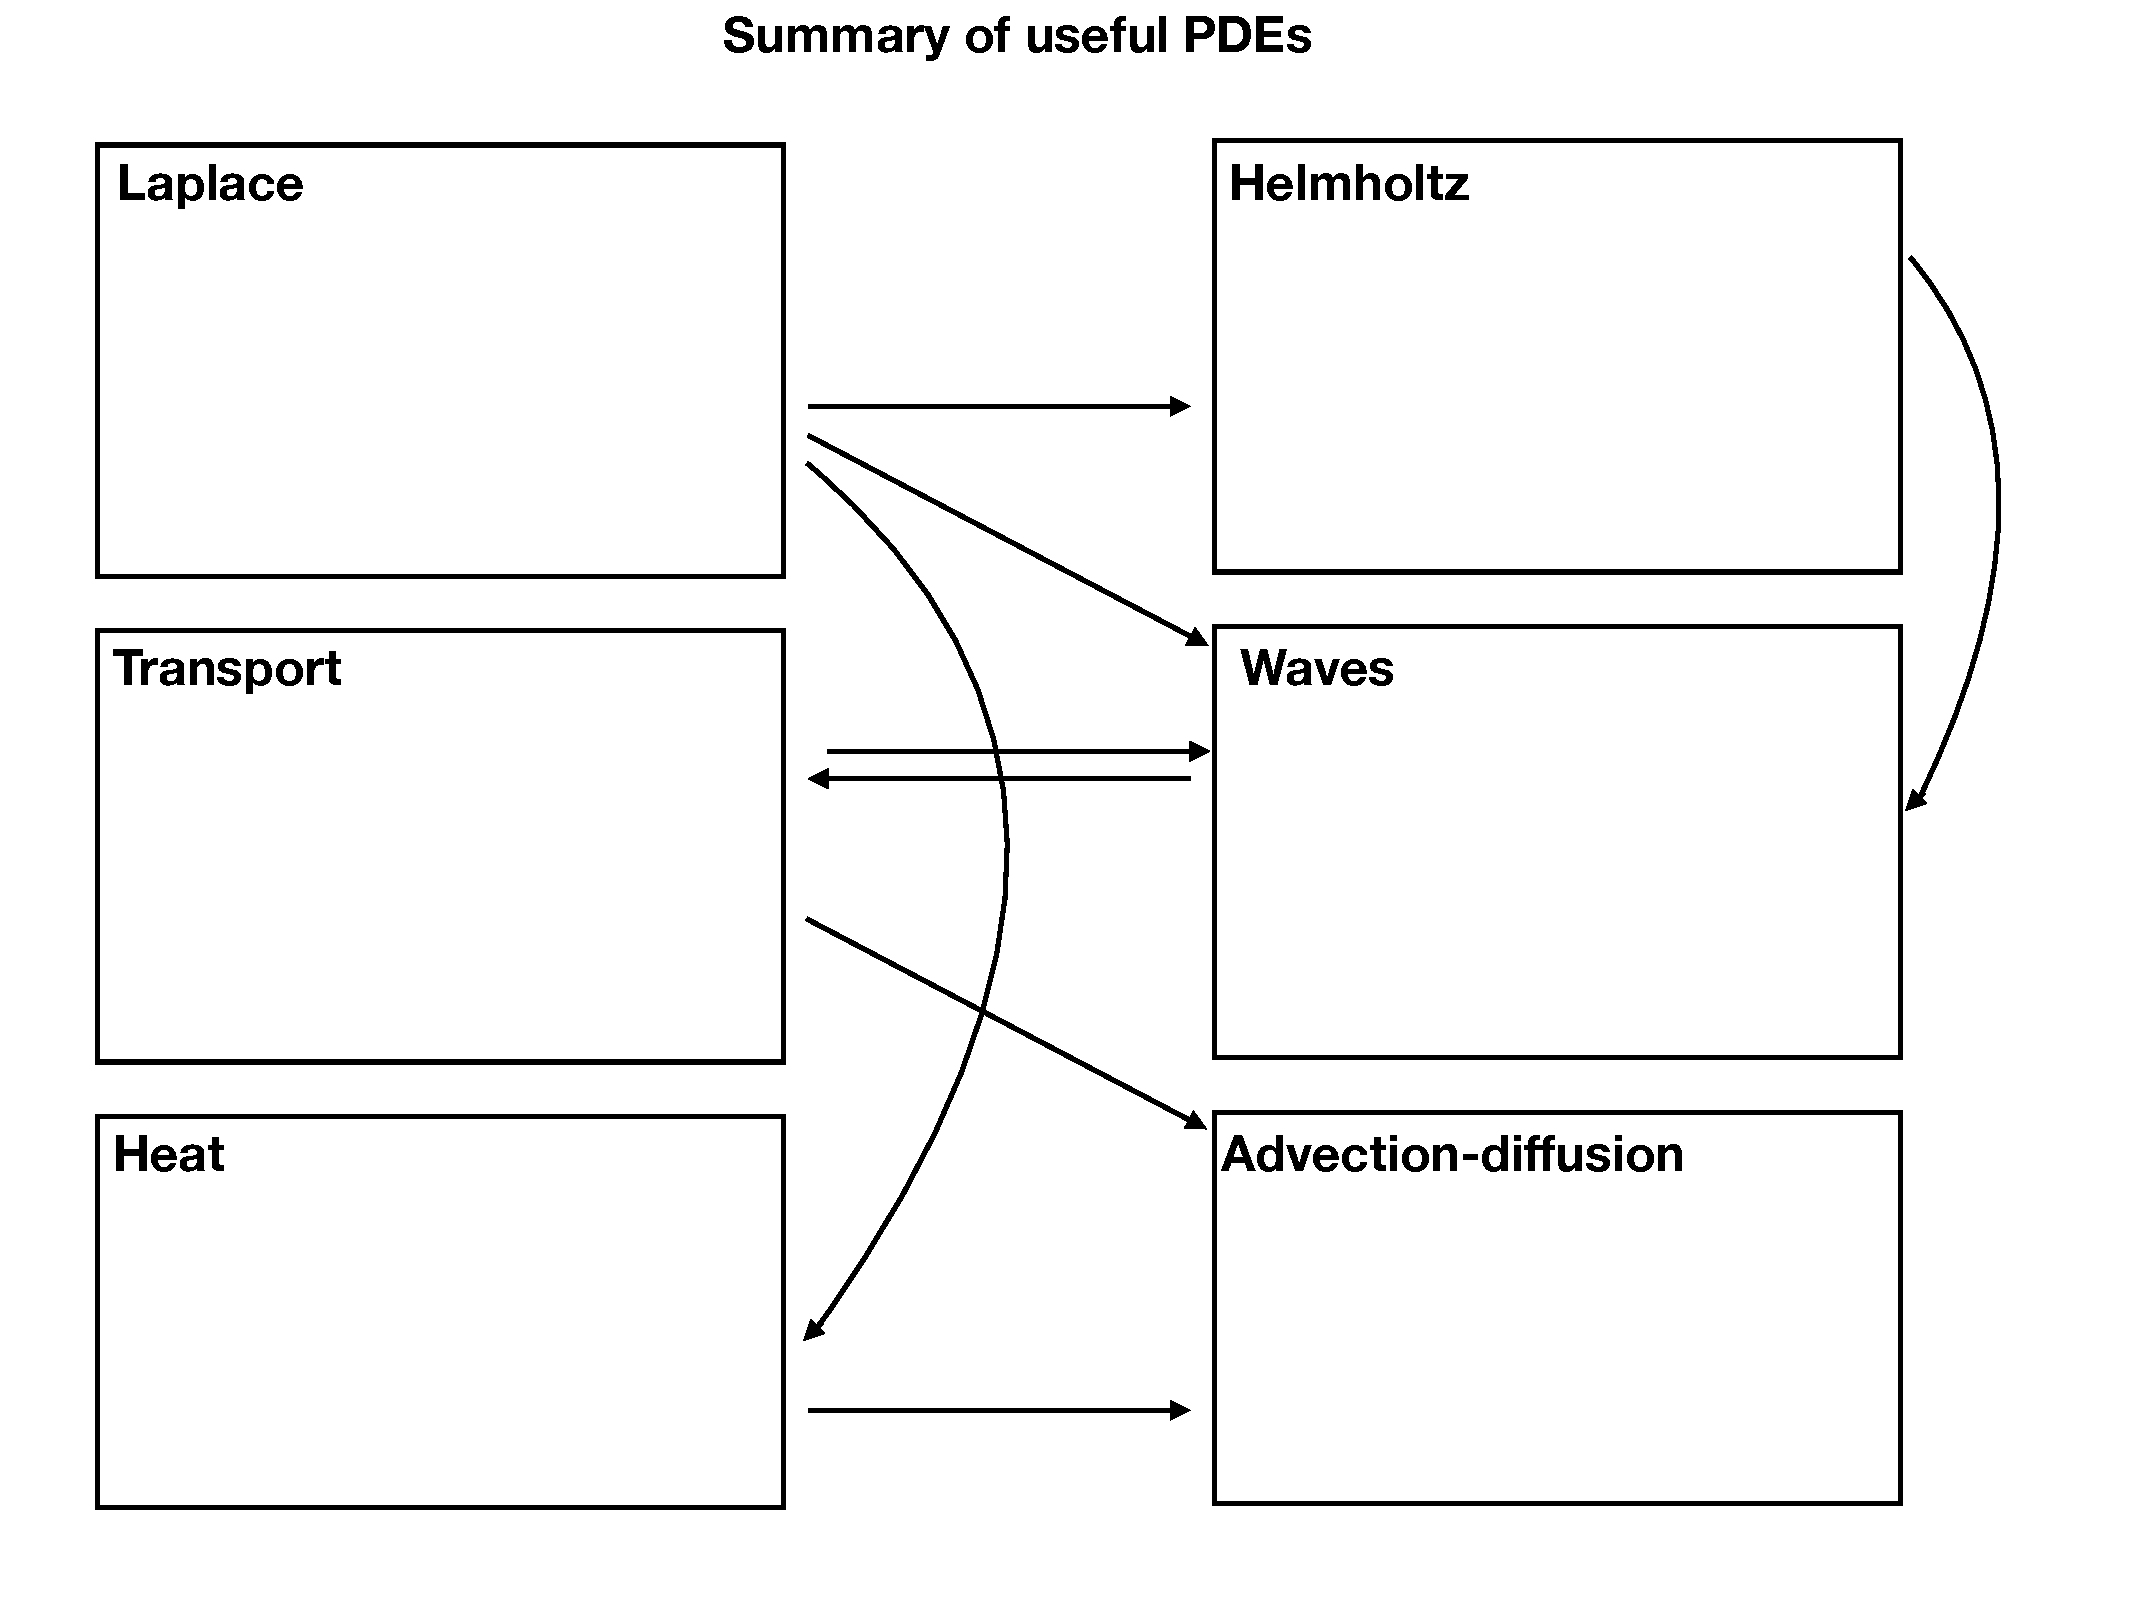
\includegraphics[width=0.9\linewidth]{img/pdes_summary.pdf}\\
  \caption{Summary of PDEs and their relationships.}
  \label{fig:pde}
 \end{figure}
 \end{Exercise}